% Options for packages loaded elsewhere
% Options for packages loaded elsewhere
\PassOptionsToPackage{unicode}{hyperref}
\PassOptionsToPackage{hyphens}{url}
\PassOptionsToPackage{dvipsnames,svgnames,x11names}{xcolor}
%
\documentclass[
]{article}
\usepackage{xcolor}
\usepackage[top=0.75in,left=0.75in,bottom=0.75in,right=0.75in]{geometry}
\usepackage{amsmath,amssymb}
\setcounter{secnumdepth}{5}
\usepackage{iftex}
\ifPDFTeX
  \usepackage[T1]{fontenc}
  \usepackage[utf8]{inputenc}
  \usepackage{textcomp} % provide euro and other symbols
\else % if luatex or xetex
  \usepackage{unicode-math} % this also loads fontspec
  \defaultfontfeatures{Scale=MatchLowercase}
  \defaultfontfeatures[\rmfamily]{Ligatures=TeX,Scale=1}
\fi
\usepackage{lmodern}
\ifPDFTeX\else
  % xetex/luatex font selection
\fi
% Use upquote if available, for straight quotes in verbatim environments
\IfFileExists{upquote.sty}{\usepackage{upquote}}{}
\IfFileExists{microtype.sty}{% use microtype if available
  \usepackage[]{microtype}
  \UseMicrotypeSet[protrusion]{basicmath} % disable protrusion for tt fonts
}{}
\makeatletter
\@ifundefined{KOMAClassName}{% if non-KOMA class
  \IfFileExists{parskip.sty}{%
    \usepackage{parskip}
  }{% else
    \setlength{\parindent}{0pt}
    \setlength{\parskip}{6pt plus 2pt minus 1pt}}
}{% if KOMA class
  \KOMAoptions{parskip=half}}
\makeatother
% Make \paragraph and \subparagraph free-standing
\makeatletter
\ifx\paragraph\undefined\else
  \let\oldparagraph\paragraph
  \renewcommand{\paragraph}{
    \@ifstar
      \xxxParagraphStar
      \xxxParagraphNoStar
  }
  \newcommand{\xxxParagraphStar}[1]{\oldparagraph*{#1}\mbox{}}
  \newcommand{\xxxParagraphNoStar}[1]{\oldparagraph{#1}\mbox{}}
\fi
\ifx\subparagraph\undefined\else
  \let\oldsubparagraph\subparagraph
  \renewcommand{\subparagraph}{
    \@ifstar
      \xxxSubParagraphStar
      \xxxSubParagraphNoStar
  }
  \newcommand{\xxxSubParagraphStar}[1]{\oldsubparagraph*{#1}\mbox{}}
  \newcommand{\xxxSubParagraphNoStar}[1]{\oldsubparagraph{#1}\mbox{}}
\fi
\makeatother

\usepackage{color}
\usepackage{fancyvrb}
\newcommand{\VerbBar}{|}
\newcommand{\VERB}{\Verb[commandchars=\\\{\}]}
\DefineVerbatimEnvironment{Highlighting}{Verbatim}{commandchars=\\\{\}}
% Add ',fontsize=\small' for more characters per line
\usepackage{framed}
\definecolor{shadecolor}{RGB}{241,243,245}
\newenvironment{Shaded}{\begin{snugshade}}{\end{snugshade}}
\newcommand{\AlertTok}[1]{\textcolor[rgb]{0.68,0.00,0.00}{#1}}
\newcommand{\AnnotationTok}[1]{\textcolor[rgb]{0.37,0.37,0.37}{#1}}
\newcommand{\AttributeTok}[1]{\textcolor[rgb]{0.40,0.45,0.13}{#1}}
\newcommand{\BaseNTok}[1]{\textcolor[rgb]{0.68,0.00,0.00}{#1}}
\newcommand{\BuiltInTok}[1]{\textcolor[rgb]{0.00,0.23,0.31}{#1}}
\newcommand{\CharTok}[1]{\textcolor[rgb]{0.13,0.47,0.30}{#1}}
\newcommand{\CommentTok}[1]{\textcolor[rgb]{0.37,0.37,0.37}{#1}}
\newcommand{\CommentVarTok}[1]{\textcolor[rgb]{0.37,0.37,0.37}{\textit{#1}}}
\newcommand{\ConstantTok}[1]{\textcolor[rgb]{0.56,0.35,0.01}{#1}}
\newcommand{\ControlFlowTok}[1]{\textcolor[rgb]{0.00,0.23,0.31}{\textbf{#1}}}
\newcommand{\DataTypeTok}[1]{\textcolor[rgb]{0.68,0.00,0.00}{#1}}
\newcommand{\DecValTok}[1]{\textcolor[rgb]{0.68,0.00,0.00}{#1}}
\newcommand{\DocumentationTok}[1]{\textcolor[rgb]{0.37,0.37,0.37}{\textit{#1}}}
\newcommand{\ErrorTok}[1]{\textcolor[rgb]{0.68,0.00,0.00}{#1}}
\newcommand{\ExtensionTok}[1]{\textcolor[rgb]{0.00,0.23,0.31}{#1}}
\newcommand{\FloatTok}[1]{\textcolor[rgb]{0.68,0.00,0.00}{#1}}
\newcommand{\FunctionTok}[1]{\textcolor[rgb]{0.28,0.35,0.67}{#1}}
\newcommand{\ImportTok}[1]{\textcolor[rgb]{0.00,0.46,0.62}{#1}}
\newcommand{\InformationTok}[1]{\textcolor[rgb]{0.37,0.37,0.37}{#1}}
\newcommand{\KeywordTok}[1]{\textcolor[rgb]{0.00,0.23,0.31}{\textbf{#1}}}
\newcommand{\NormalTok}[1]{\textcolor[rgb]{0.00,0.23,0.31}{#1}}
\newcommand{\OperatorTok}[1]{\textcolor[rgb]{0.37,0.37,0.37}{#1}}
\newcommand{\OtherTok}[1]{\textcolor[rgb]{0.00,0.23,0.31}{#1}}
\newcommand{\PreprocessorTok}[1]{\textcolor[rgb]{0.68,0.00,0.00}{#1}}
\newcommand{\RegionMarkerTok}[1]{\textcolor[rgb]{0.00,0.23,0.31}{#1}}
\newcommand{\SpecialCharTok}[1]{\textcolor[rgb]{0.37,0.37,0.37}{#1}}
\newcommand{\SpecialStringTok}[1]{\textcolor[rgb]{0.13,0.47,0.30}{#1}}
\newcommand{\StringTok}[1]{\textcolor[rgb]{0.13,0.47,0.30}{#1}}
\newcommand{\VariableTok}[1]{\textcolor[rgb]{0.07,0.07,0.07}{#1}}
\newcommand{\VerbatimStringTok}[1]{\textcolor[rgb]{0.13,0.47,0.30}{#1}}
\newcommand{\WarningTok}[1]{\textcolor[rgb]{0.37,0.37,0.37}{\textit{#1}}}

\usepackage{longtable,booktabs,array}
\newcounter{none} % for unnumbered tables
\usepackage{calc} % for calculating minipage widths
% Correct order of tables after \paragraph or \subparagraph
\usepackage{etoolbox}
\makeatletter
\patchcmd\longtable{\par}{\if@noskipsec\mbox{}\fi\par}{}{}
\makeatother
% Allow footnotes in longtable head/foot
\IfFileExists{footnotehyper.sty}{\usepackage{footnotehyper}}{\usepackage{footnote}}
\makesavenoteenv{longtable}
\usepackage{graphicx}
\makeatletter
\newsavebox\pandoc@box
\newcommand*\pandocbounded[1]{% scales image to fit in text height/width
  \sbox\pandoc@box{#1}%
  \Gscale@div\@tempa{\textheight}{\dimexpr\ht\pandoc@box+\dp\pandoc@box\relax}%
  \Gscale@div\@tempb{\linewidth}{\wd\pandoc@box}%
  \ifdim\@tempb\p@<\@tempa\p@\let\@tempa\@tempb\fi% select the smaller of both
  \ifdim\@tempa\p@<\p@\scalebox{\@tempa}{\usebox\pandoc@box}%
  \else\usebox{\pandoc@box}%
  \fi%
}
% Set default figure placement to htbp
\def\fps@figure{htbp}
\makeatother


% definitions for citeproc citations
\NewDocumentCommand\citeproctext{}{}
\NewDocumentCommand\citeproc{mm}{%
  \begingroup\def\citeproctext{#2}\cite{#1}\endgroup}
\makeatletter
 % allow citations to break across lines
 \let\@cite@ofmt\@firstofone
 % avoid brackets around text for \cite:
 \def\@biblabel#1{}
 \def\@cite#1#2{{#1\if@tempswa , #2\fi}}
\makeatother
\newlength{\cslhangindent}
\setlength{\cslhangindent}{1.5em}
\newlength{\csllabelwidth}
\setlength{\csllabelwidth}{3em}
\newenvironment{CSLReferences}[2] % #1 hanging-indent, #2 entry-spacing
 {\begin{list}{}{%
  \setlength{\itemindent}{0pt}
  \setlength{\leftmargin}{0pt}
  \setlength{\parsep}{0pt}
  % turn on hanging indent if param 1 is 1
  \ifodd #1
   \setlength{\leftmargin}{\cslhangindent}
   \setlength{\itemindent}{-1\cslhangindent}
  \fi
  % set entry spacing
  \setlength{\itemsep}{#2\baselineskip}}}
 {\end{list}}
\usepackage{calc}
\newcommand{\CSLBlock}[1]{\hfill\break\parbox[t]{\linewidth}{\strut\ignorespaces#1\strut}}
\newcommand{\CSLLeftMargin}[1]{\parbox[t]{\csllabelwidth}{\strut#1\strut}}
\newcommand{\CSLRightInline}[1]{\parbox[t]{\linewidth - \csllabelwidth}{\strut#1\strut}}
\newcommand{\CSLIndent}[1]{\hspace{\cslhangindent}#1}



\setlength{\emergencystretch}{3em} % prevent overfull lines

\providecommand{\tightlist}{%
  \setlength{\itemsep}{0pt}\setlength{\parskip}{0pt}}



 


\usepackage{amsmath}
\usepackage[dvipsnames]{xcolor}
\usepackage[shortlabels]{enumitem}
\usepackage{parskip}
\usepackage{hyperref}
\usepackage{geometry}
\usepackage{float}
\makeatletter
\@ifpackageloaded{caption}{}{\usepackage{caption}}
\AtBeginDocument{%
\ifdefined\contentsname
  \renewcommand*\contentsname{Table of contents}
\else
  \newcommand\contentsname{Table of contents}
\fi
\ifdefined\listfigurename
  \renewcommand*\listfigurename{List of Figures}
\else
  \newcommand\listfigurename{List of Figures}
\fi
\ifdefined\listtablename
  \renewcommand*\listtablename{List of Tables}
\else
  \newcommand\listtablename{List of Tables}
\fi
\ifdefined\figurename
  \renewcommand*\figurename{Figure}
\else
  \newcommand\figurename{Figure}
\fi
\ifdefined\tablename
  \renewcommand*\tablename{Table}
\else
  \newcommand\tablename{Table}
\fi
}
\@ifpackageloaded{float}{}{\usepackage{float}}
\floatstyle{ruled}
\@ifundefined{c@chapter}{\newfloat{codelisting}{h}{lop}}{\newfloat{codelisting}{h}{lop}[chapter]}
\floatname{codelisting}{Listing}
\newcommand*\listoflistings{\listof{codelisting}{List of Listings}}
\makeatother
\makeatletter
\makeatother
\makeatletter
\@ifpackageloaded{caption}{}{\usepackage{caption}}
\@ifpackageloaded{subcaption}{}{\usepackage{subcaption}}
\makeatother
\usepackage{bookmark}
\IfFileExists{xurl.sty}{\usepackage{xurl}}{} % add URL line breaks if available
\urlstyle{same}
\hypersetup{
  pdftitle={Lab One -- Installing R{,} Positron{,} and tinytex},
  colorlinks=true,
  linkcolor={blue},
  filecolor={Maroon},
  citecolor={Blue},
  urlcolor={Blue},
  pdfcreator={LaTeX via pandoc}}


\title{Lab One -- Installing R, Positron, and tinytex}
\author{}
\date{}
\begin{document}
\maketitle


\normalsize

\normalsize

\section{Install Software}\label{install-software}

\begin{itemize}
\tightlist
\item
  \href{https://cran.r-project.org/}{Install R}.
\item
  \href{https://positron.posit.co/download.html}{Install Positron}.
\item
  \href{https://yihui.org/tinytex/}{Install tinytex}.
\end{itemize}

\section{Set Up GitHub}\label{set-up-github}

\begin{itemize}
\tightlist
\item
  \href{https://github.com/}{Sign Up for GitHub}.
\item
  Sign Up for
  \href{https://classroom.github.com/classrooms/156721198-colgateuniversitycipolli-sp2026-math240}{Our
  GitHub Classroom}.
\item
  Pull the GitHub Repo for Lab One
  \href{https://classroom.github.com/a/8jPlfX90}{here}.
\end{itemize}

\section{Compile the Lab Template}\label{compile-the-lab-template}

\begin{itemize}
\tightlist
\item
  Compile the Lab One template as an html file (default).
\item
  Use the commented code to compile the Lab One template as a pdf file.
\end{itemize}

\section{Learn to Use Quarto and R}\label{learn-to-use-quarto-and-r}

\begin{itemize}
\tightlist
\item
  Recreate this section in your \textbf{\texttt{Lab1WriteUp.qmd}} file.
\end{itemize}

\subsection{Bold, Italics, Underline}\label{bold-italics-underline}

\textbf{This is bold text}

\emph{This is italicized text}

This is underlined text

\subsection{Lists and Enumerated
Lists}\label{lists-and-enumerated-lists}

\begin{itemize}
\tightlist
\item
  This is item one

  \begin{itemize}
  \tightlist
  \item
    This is item a
  \item
    This is item b
  \end{itemize}
\item
  This is item two
\item
  This is item three

  \begin{itemize}
  \tightlist
  \item
    This is item c
  \item
    This is item d
  \item
    This is item e
  \end{itemize}
\item
  This is item four
\end{itemize}

\begin{enumerate}
\def\labelenumi{\arabic{enumi}.}
\tightlist
\item
  This is item one

  \begin{enumerate}
  \def\labelenumii{\alph{enumii}.}
  \tightlist
  \item
    This is item a
  \item
    This is item b
  \item
    This is item c
  \end{enumerate}
\item
  This is item two
\item
  This is item three
\item
  This is item four
\end{enumerate}

\subsection{Math}\label{math}

The quadratic formula \begin{align*}
x = \frac{-b \pm \sqrt{b^2-4ac}}{2a}.
\end{align*} It is helpful for solving equations like \begin{align*}
x^2+2x-13=0.
\end{align*} Using \(a=1,b=2,c=-13,\) we find solutions using the
quadratic formula. \begin{align*}
x &= \frac{-b \pm \sqrt{b^2-4ac}}{2a} \tag{Definition} \\
&= \frac{-(2) \pm \sqrt{(2)^2-4(1)-13}}{2(1)} \tag{Definition} \\
&= \frac{-2 \pm \sqrt{56}}{2} \tag{Symplifying} \\
&= \frac{-2}{2} \pm \frac{\sqrt{56}}{2} \tag{Rewriting} \\
&= \frac{-2}{2} \pm \sqrt{\frac{56}{4} \tag{Rewriting} }\\
&= -1 \pm \sqrt{14} \tag{Symplifying} \\
&= -4.741657 \text{ or } 2.741657
\end{align*}

\subsection{Figures}\label{figures}

We can \emph{show} we've found the correct answer by plotting the line
and the points (see Figure~\ref{fig-one-quadratic}).

\scriptsize

\begin{Shaded}
\begin{Highlighting}[numbers=left,,]
\NormalTok{dat }\OtherTok{\textless{}{-}} \FunctionTok{tibble}\NormalTok{(}\AttributeTok{x=}\FunctionTok{seq}\NormalTok{(}\SpecialCharTok{{-}}\DecValTok{6}\NormalTok{, }\DecValTok{6}\NormalTok{, }\AttributeTok{length.out=}\DecValTok{1000}\NormalTok{))}\SpecialCharTok{|\textgreater{}}
              \FunctionTok{mutate}\NormalTok{(}\AttributeTok{y =}\NormalTok{ x}\SpecialCharTok{\^{}}\DecValTok{2} \SpecialCharTok{+} \DecValTok{2}\SpecialCharTok{*}\NormalTok{x }\SpecialCharTok{{-}}\DecValTok{13}\NormalTok{)}

\FunctionTok{ggplot}\NormalTok{(}\AttributeTok{data=}\NormalTok{dat)}\SpecialCharTok{+}
      \FunctionTok{geom\_line}\NormalTok{(}\FunctionTok{aes}\NormalTok{(}\AttributeTok{x=}\NormalTok{x, }\AttributeTok{y=}\NormalTok{y))}\SpecialCharTok{+}
      \FunctionTok{geom\_hline}\NormalTok{(}\AttributeTok{yintercept=}\DecValTok{0}\NormalTok{, }\AttributeTok{alpha=}\FloatTok{0.50}\NormalTok{)}\SpecialCharTok{+}
      \FunctionTok{geom\_vline}\NormalTok{(}\AttributeTok{xintercept=}\DecValTok{0}\NormalTok{, }\AttributeTok{alpha=}\FloatTok{0.50}\NormalTok{)}\SpecialCharTok{+}
      \FunctionTok{theme\_bw}\NormalTok{()}\SpecialCharTok{+}
      \FunctionTok{labs}\NormalTok{(}\AttributeTok{x=}\StringTok{"x"}\NormalTok{, }\AttributeTok{y=}\StringTok{"y"}\NormalTok{)}\SpecialCharTok{+}
      \FunctionTok{annotate}\NormalTok{(}\StringTok{"point"}\NormalTok{, }\AttributeTok{x=}\SpecialCharTok{{-}}\DecValTok{1}\SpecialCharTok{{-}}\FunctionTok{sqrt}\NormalTok{(}\DecValTok{14}\NormalTok{), }\AttributeTok{y=}\DecValTok{0}\NormalTok{, }\AttributeTok{color=}\StringTok{"red"}\NormalTok{)}\SpecialCharTok{+}
      \FunctionTok{annotate}\NormalTok{(}\StringTok{"point"}\NormalTok{, }\AttributeTok{x=}\SpecialCharTok{{-}}\DecValTok{1}\SpecialCharTok{+}\FunctionTok{sqrt}\NormalTok{(}\DecValTok{14}\NormalTok{), }\AttributeTok{y=}\DecValTok{0}\NormalTok{, }\AttributeTok{color=}\StringTok{"red"}\NormalTok{)}
\end{Highlighting}
\end{Shaded}

\begin{figure}[H]

\caption{\label{fig-one-quadratic}Graph of the quadratic.}

\centering{

\pandocbounded{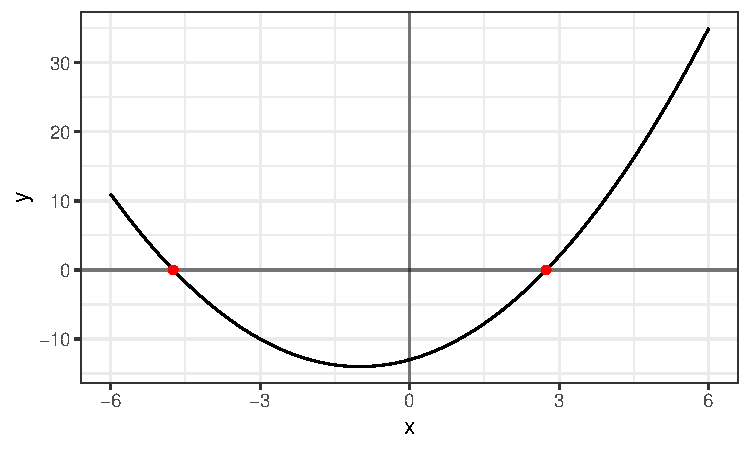
\includegraphics[keepaspectratio]{Lab1WriteUp_files/figure-pdf/fig-one-quadratic-1.pdf}}

}

\end{figure}%

\normalsize

\subsection{Tables}\label{tables}

Note, we can pick points to show intermediate value theorem, noting that
our function is continuous. For example, in Table~\ref{tbl-points}, we
can see there must be a root between \(x = -5\) and \(x = 0\) and
another between \(x=0\) and \(x=5\).

\scriptsize

\begin{Shaded}
\begin{Highlighting}[numbers=left,,]
\FunctionTok{tibble}\NormalTok{(}\AttributeTok{x =} \FunctionTok{c}\NormalTok{(}\SpecialCharTok{{-}}\DecValTok{5}\NormalTok{, }\SpecialCharTok{{-}}\DecValTok{1}\SpecialCharTok{{-}}\FunctionTok{sqrt}\NormalTok{(}\DecValTok{14}\NormalTok{), }\DecValTok{0}\NormalTok{, }\SpecialCharTok{{-}}\DecValTok{1}\SpecialCharTok{+}\FunctionTok{sqrt}\NormalTok{(}\DecValTok{14}\NormalTok{), }\DecValTok{5}\NormalTok{)) }\SpecialCharTok{|\textgreater{}}
      \FunctionTok{mutate}\NormalTok{(}\AttributeTok{y =}\NormalTok{ x}\SpecialCharTok{\^{}}\DecValTok{2} \SpecialCharTok{+} \DecValTok{2}\SpecialCharTok{*}\NormalTok{x }\SpecialCharTok{{-}}\DecValTok{13}\NormalTok{)}\SpecialCharTok{|\textgreater{}}
\NormalTok{      knitr}\SpecialCharTok{::}\FunctionTok{kable}\NormalTok{(}\AttributeTok{digits=}\DecValTok{4}\NormalTok{)}
\end{Highlighting}
\end{Shaded}

{

\begin{longtable}[]{@{}rr@{}}

\caption{\label{tbl-points}Table of values of the quadratic.}

\tabularnewline

\toprule\noalign{}
x & y \\
\midrule\noalign{}
\endhead
\bottomrule\noalign{}
\endlastfoot
-5.0000 & 2 \\
-4.7417 & 0 \\
0.0000 & -13 \\
2.7417 & 0 \\
5.0000 & 22 \\

\end{longtable}

}

\normalsize

\subsection{Citations}\label{citations}

Above, I used the \texttt{tidyverse} package (Wickham et al. 2019) to
create Figure~\ref{fig-one-quadratic} and Table~\ref{tbl-points}.
Additionally, I used the \texttt{knitr} package (Xie 2025) to nicely
format the table.

Note that you can ask for citations for \textbf{\texttt{R}} packages
using the \textbf{\texttt{citation()}} function.

\subsection{Delivery}\label{delivery}

Ensure to render the full project using the following code, so the PDF
link will work and a .pdf file will be created.

\subsection{References}\label{references}

\section*{References}\label{bibliography}
\addcontentsline{toc}{section}{References}

\protect\phantomsection\label{refs}
\begin{CSLReferences}{1}{1}
\bibitem[\citeproctext]{ref-tidyverse}
Wickham, Hadley, Mara Averick, Jennifer Bryan, et al. 2019. {``Welcome
to the {tidyverse}.''} \emph{Journal of Open Source Software} 4 (43):
1686. \url{https://doi.org/10.21105/joss.01686}.

\bibitem[\citeproctext]{ref-knitr}
Xie, Yihui. 2025. \emph{A General-Pupose Package for Dynamic Report
Generation in r.} \url{https://yihui.org/knitr/}.

\end{CSLReferences}




\end{document}
